\section{Hardware Implementations}

Below are three possible implementations. A designer could choose one, mix and
match, or come up with their own design.

\subsection{Direct}

\begin{figure}
   \centering
   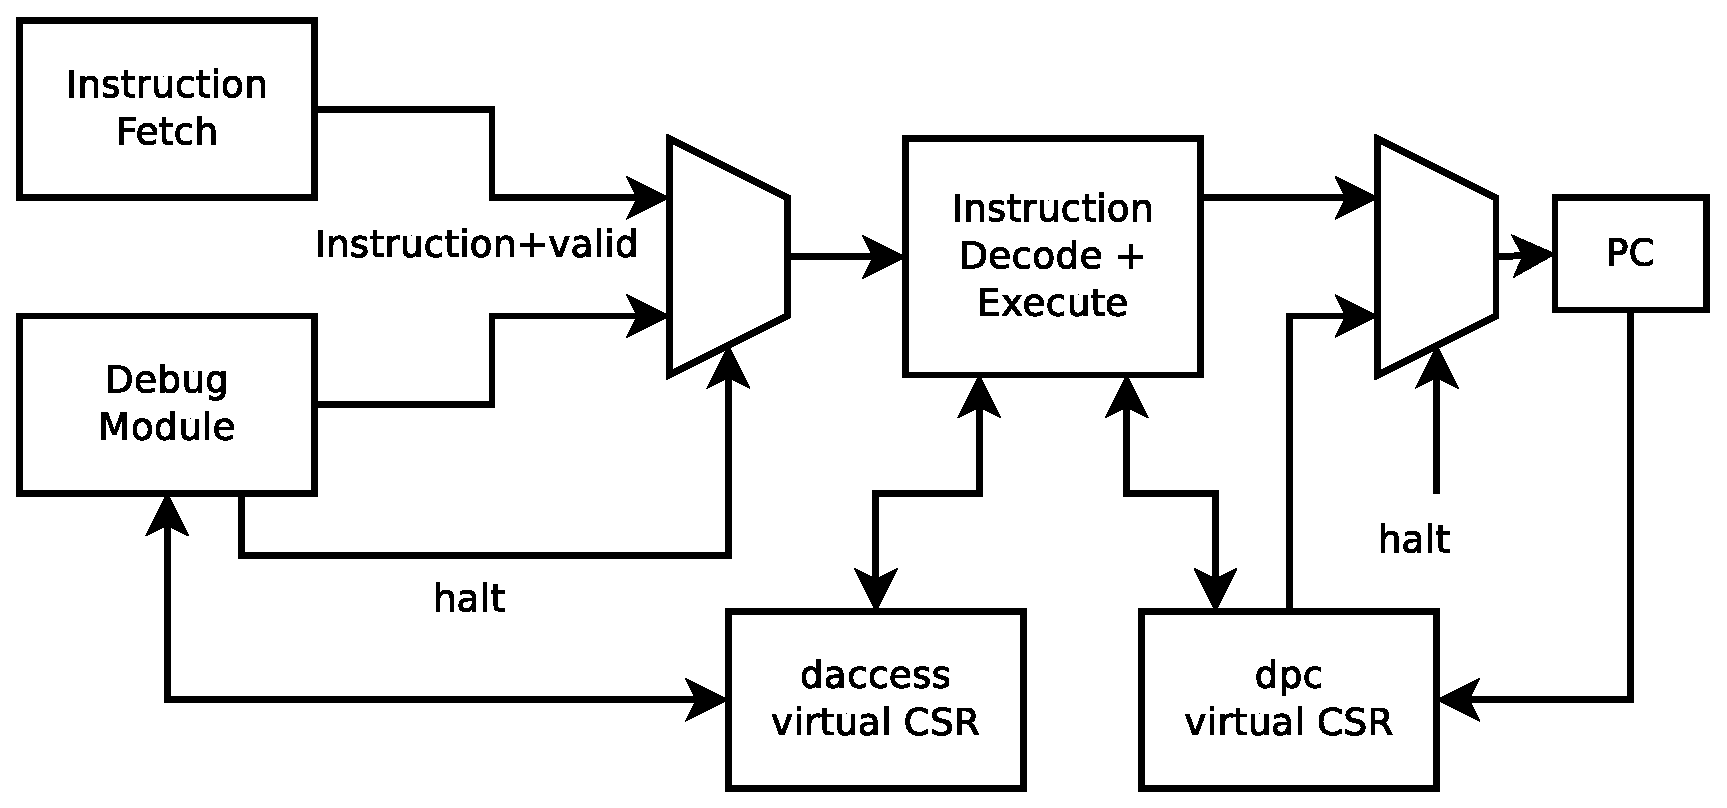
\includegraphics[width=\textwidth]{direct.eps}
   \caption{Direct Implementation}
   \label{fig:direct}
\end{figure}

Figure~\ref{fig:direct} shows an implementation that might be appropriate for
small cores.  In this implementation the DM reaches directly into the core's
pipeline to push instructions. Entering halt mode might stall the pipeline, or
send bubbles through. Data exchange happens by accessing a special CSR.
Incrementing the PC is inhibited so no separate register is needed to store the
PC. Instead accessing \Rdpc modifies the actual PC register.  When the halt is
deasserted, regular instruction execution resumes.

\subsection{Instruction Fetch}

In this implementation, just the instruction fetch unit is changed. In halt
mode the unit simply starts fetching instructions from the DM, while the PC is
unchanged. The DM could wait until the debugger gives it an instruction before
completing an access, or it could immediately return a jump-to-self instruction
if the debugger hasn't given it an instruction. Data exchange probably happens
through a special memory address. \Rdpc maps to the actual PC. When the debug
interrupt is deasserted, regular instruction execution resumes at the current
PC.

\subsection{Plain Exception}

\begin{figure}
   \centering
   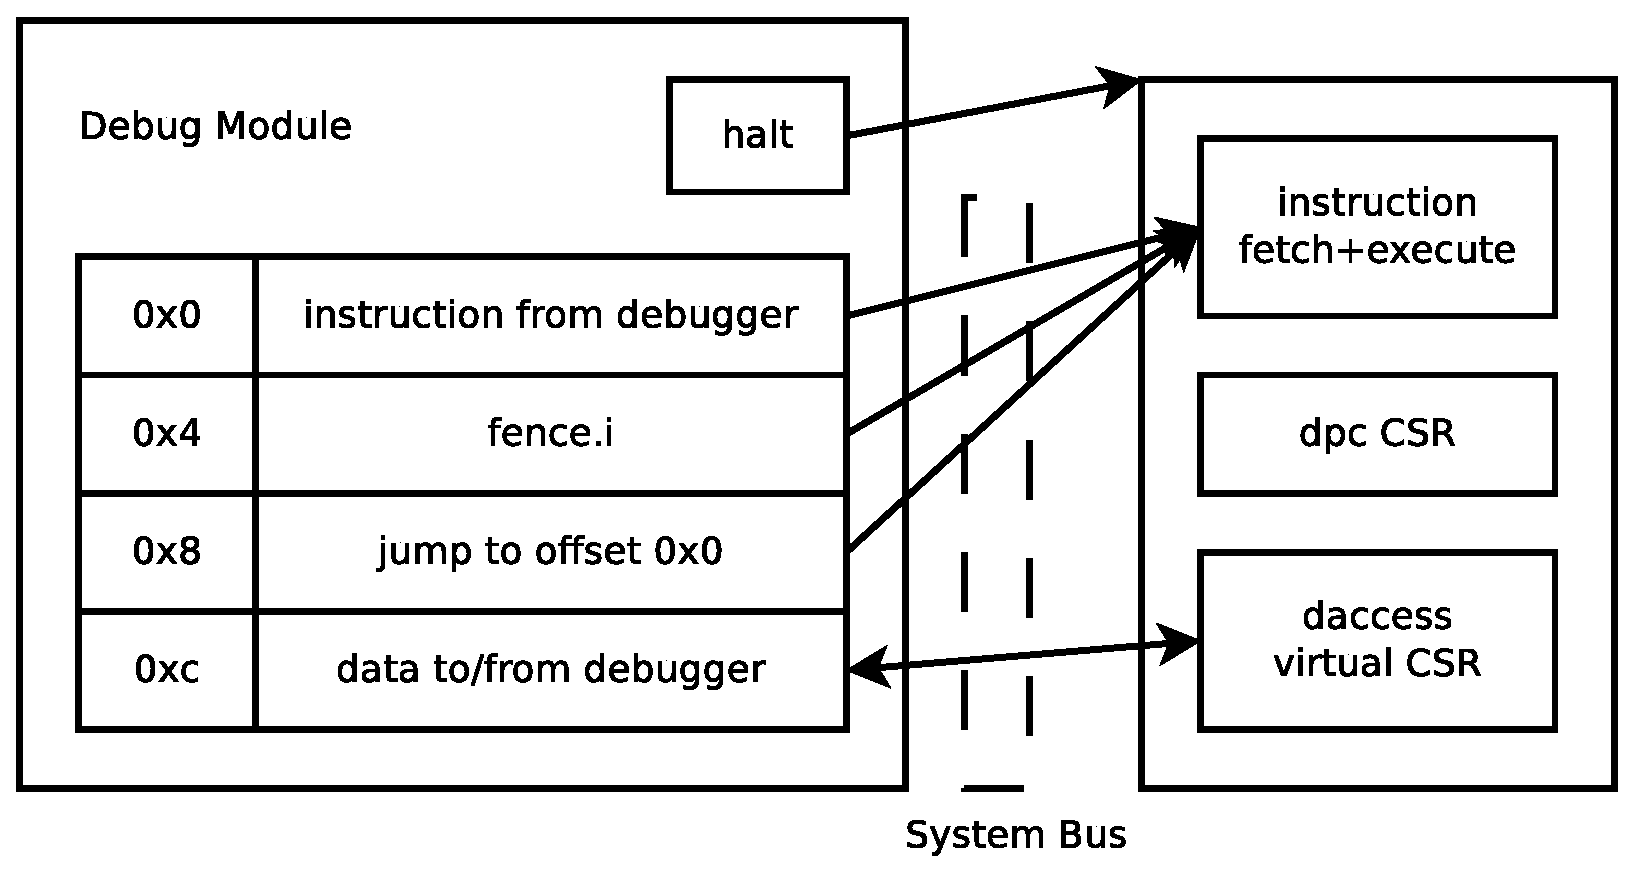
\includegraphics[width=\textwidth]{plain-exception.eps}
   \caption{Plain Exception Implementation}
   \label{fig:direct}
\end{figure}

In this implementation, being halted acts more like a real exception, jumping
to a memory region that is serviced by the DM. The PC is saved to \Rdpc. Any
details required to make the core behave correctly (eg.  executing fence.i when
a new instruction is mapped to some address) could be handled by a Debug ROM in
the DM. When the debug interrupt is deasserted, the DM feeds the hart a dret
instruction, which causes the PC to be restored and normal execution to resume.
Data is probably exchanged through a memory address.

In single-hart systems, the DM can just keep an instruction fetch access alive
until the debugger has data for it.  In multi-core systems, the DM must have
some way of allowing the debugger to choose which halted hart to send
instructions to. It could keep multiple fetches alive, or immediately return a
jump-to-self for harts that aren't the currently selected one. If it does that,
it must pretend to the debugger that there is an access pending. In the process
it assumes that a hart is going to keep fetching instructions, and won't
suddenly go to sleep or be powered down.
